\documentclass[12pt]{article}
\usepackage{amsmath,amssymb,amsthm}
\usepackage{graphicx,mathabx}
\usepackage{xcolor}
\usepackage{tikz}
\usepackage{placeins}
\usepackage{lipsum}
\usepackage{mathtools}
\usepackage[shortlabels]{enumitem}
\usepackage{wrapfig}
\DeclarePairedDelimiter{\ceil}{\lceil}{\rceil}
\begin{document}
\title{TCSS 343 - Week 1 - Tuesday}
\author{Jake McKenzie}
\maketitle
\noindent\centerline{\textbf{Asymptotics with Mathematical Induction}}\\\\\\\\\\\\\\\\
\begin{center}
    ``Programs must be written for people to read, and only incidentally for machines to execute". \\$\cdots$\\ Harold Abelson
\end{center}
\begin{center}
    ``You shouldn't try optimizing something that you can't measure." \\$\cdots$\\ Elecia White
\end{center}
\begin{center}
    ``People worry that computers will get too smart and take over the world, but the real problem is that they're too stupid and they've already taken over the world." \\$\cdots$\\ Pedro Domingos
\end{center}
\newpage
Exact answers are nice when you can find them. Often times we can't or don't care to find them. As computer scientists we care about the behavior of the algorithms we employ. If we run into a recurrence relation or summation that expressed loosly the behaivor of these algorithms we'd like to know something about their runtime.\\\\
\centerline{\textbf{Asymptotic Notation in Seven Words:}}\\
\centerline{\textbf{suppress constant factors and lower-order terms}}\\\\
Constant factors are things that will be language and system dependent while lower order terms are irrelevant for large inputs.\\\\
Now consider these definitions:\\
\textbf{Big-O Notation}\\
If $\lim\limits_{n\to\infty}{\frac{f(n)}{g(n)}}\to0$ then $f(n) \in O(g(n))$\\\\
This is another way of saying that $f(n) \leq c \cdot g(n)$ for some position $c$.\\
\textbf{Big-$\Omega$ Notation}\\
If $\lim\limits_{n\to\infty}{\frac{f(n)}{g(n)}}\to\infty$ then $f(n) \in \Omega(g(n))$\\\\
This is another way of saying that $f(n) \geq c \cdot g(n)$ for some position $c$.\\
\textbf{Big-$\Theta$ Notation}\\
If $\lim\limits_{n\to\infty}{\frac{f(n)}{g(n)}}\to k$ where k is a positive finite number then $f(n) \in \Theta(g(n))$\\\\
This is another way of saying that $f(n) \in O(g(n))$ and $f(n) \in \Omega(g(n))$\.\\
Now while we're in this course, we will typically need to show that these relationships are true when prompted, but it's always good to know that the following is true where \begin{math}0 < \epsilon < 1 < c\end{math}.\\
\[1 < \log{\log{n}} < \log{n} < n^{\epsilon} < n^c < n^{log{n}} < c^n < n^n < c^{c^{n}}\]\\
This asymptotic pecking order above is from Don Knuth's Concrete Mathematics.\\\\
\newpage
From Tim Roughgarden's Algorithms Illuminated: \\
$$\max\{f(n),g(n)\} \leq f(n) + g(n) \land  2 \cdot \max\{f(n),g(n)\} \geq f(n) + g(n)$$
(reminder that $\land$ is the logical ``and" symbol.)\\\\
\begin{enumerate}
\item[0. ] Show the following by using the definition of big Theta and the information immediately above to show that $\max\{f(n),g(n)\}\in\Theta(f(n) + g(n))$
\newpage
\item Arrange the following functions in order of increasing growth rate, with $g(n)$ following $f(n)$ 
in your list if and only if $f(n) \in O(g(n))$. That means using the limit definitions I gave you or by proof 
technique you've seen in class. You cannot simply use Don's asymptotic pecking order I stated but I strongly 
suggest you use the asymptotic pecking order as a guide to the neighborhood of a correct answer.\\
\begin{enumerate}[a)]
\item $\sum\limits_{i = 0}^{n} 2^i$\\
\item $n^2$\\
\item $n^{0.9999999}\log{n}$\\
\item $1.00001^n$\\
\item $4^{\log{n}}$\\
\item $100^{\sqrt{n}}$\\
\item $\log{2^{\frac{n}{2}}}$\\
\item $1000000n$\\
\end{enumerate}
\newpage
\item Arrange the following functions in order of increasing growth rate, with $g(n)$ following $f(n)$ in your list if and only if $f(n) \in O(g(n))$. That means using the limit definitions I gave you or by proof technique you've seen in class. You cannot simply use Don's asymptotic pecking order I stated but I strongly suggest you use the asymptotic pecking order as a guide to the neighborhood of a correct answer.\\
\begin{enumerate}[a)]
\item  $n^{\frac{5}{3}}$\\
\item $\sum\limits_{i = 0}^{n} (i + 1)$\\
\item $n\sqrt{n}$\\
\item $\log{n^n}$\\
\item $(\frac{n}{\log{n}})^3$\\
\item  $2^{\frac{n}{2}}$\\
\item  $\log{\log{n}}$\\
\item  $n^{1.5}$\\
\end{enumerate}
\newpage
\item Prove by induction that: $\sum\limits_{k=1}^{n}{\frac{k}{2^k}}=2-2^{1-n}-n2^{-n}$.
\newpage
\item The \textbf{pigeonhole principle} (in one of its more simple variations states: 
If you have $n$ pigeons in $h$ holes, then ``some hole'' has $\ge \ceil{\frac{n}{h}}$ pigeons. 
Prove this principle by strong induction. (Hint: What does $\frac{n}{h}$ represent mathematically?)
\newpage
\centerline{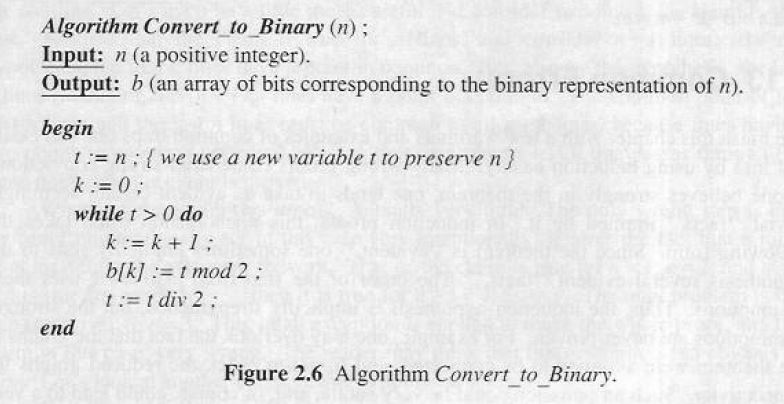
\includegraphics[scale = 0.6]{algo.jpg}}
\item For the following problem we will explore an induction and the
notion of an \textbf{invariant} of an algorithm, which put simply, is a statement about
a variable correct independent of the number of times a loop is executed. For the purposes of 
this algorithm the expression: $n = t \times 2^k + m$ is a loop invariant. Loop invariants can 
be hard to find but are often the heart of any algorithm.\\
\textbf{Induction Hypothesis: } if $m$ is the integer represented by 
the binary array $b[1\dots k]$, then $n = t \times 2^k + m$. To prove the 
correctness of this algorithm we must prove three conditions:
\begin{enumerate}
\item The hypothesis is true at the beginning of the loop.
\item The truth of the hypothesis at steps $k$ implies the step $k+1$.
\item When the loop terminates, the hypothesis implies the correctness of the algorithm.
\end{enumerate}
Attempt to complete the proof given the information I've given you to start. 
\end{enumerate}
\end{document}